
% Title --> Balance control strategy for legged robots with complaint contacts
% This can go for T3.4

During the second year, UB proposed an algorithm for implementing a momentum
based controller to control balancing motion of legged robots with non-rigid
contacts with the environments \cite{Azad&Mistry15}.  The proposed strategy
converts the balance problem to a linear constrained optimization problem
which its output is the vector of desired joint accelerations.  It first
calculates the desired supporting forces at the contact points by using the
robot’s momentum.  Then, based on the contact model and by using the Jacobian
of the contact points, it converts the desired contact forces to the desired
joint accelerations.  At the end, by using the inverse dynamics of the robot,
the joint torques are calculated.  To implement the proposed method in
practice, stiffness and damping coefficients of the contact model have to be
estimated beforehand by using contact model parameter estimation methods.


% Title --> An experimental study of robot control during environmental
% contacts based on projected operational space dynamics
% This can go for either T3.3 or T3.4

UB also studied the problem of constrained motion for a manipulator performing
a task while in contact with the environment, and proposed a solution based on
projected operational space dynamics \cite{Ortenzietal14}.  The main
advantages of this control technique are: 1) it exploits the environment
contact constraint itself, so as to minimise the joint torques needed to
perform the task; 2) it enables full decoupling of motion and force control;
3) force feedback from a force sensor mounted at the end effector or other
contact points is not needed.  This work is a step towards a robot control
strategy which mimics the human behaviour of exploiting contacts with the
environment to help perform tasks.  They also presented an experimental
implementation of the control method in which a KUKA LWR IV manipulator used
an eraser to wipe a whiteboard.  They showed that the proposed controller can
effectively exploit contact with the whiteboard in order to reduce joint
torques while still performing the desired wiping motion.

\begin{figure}
  \centering
  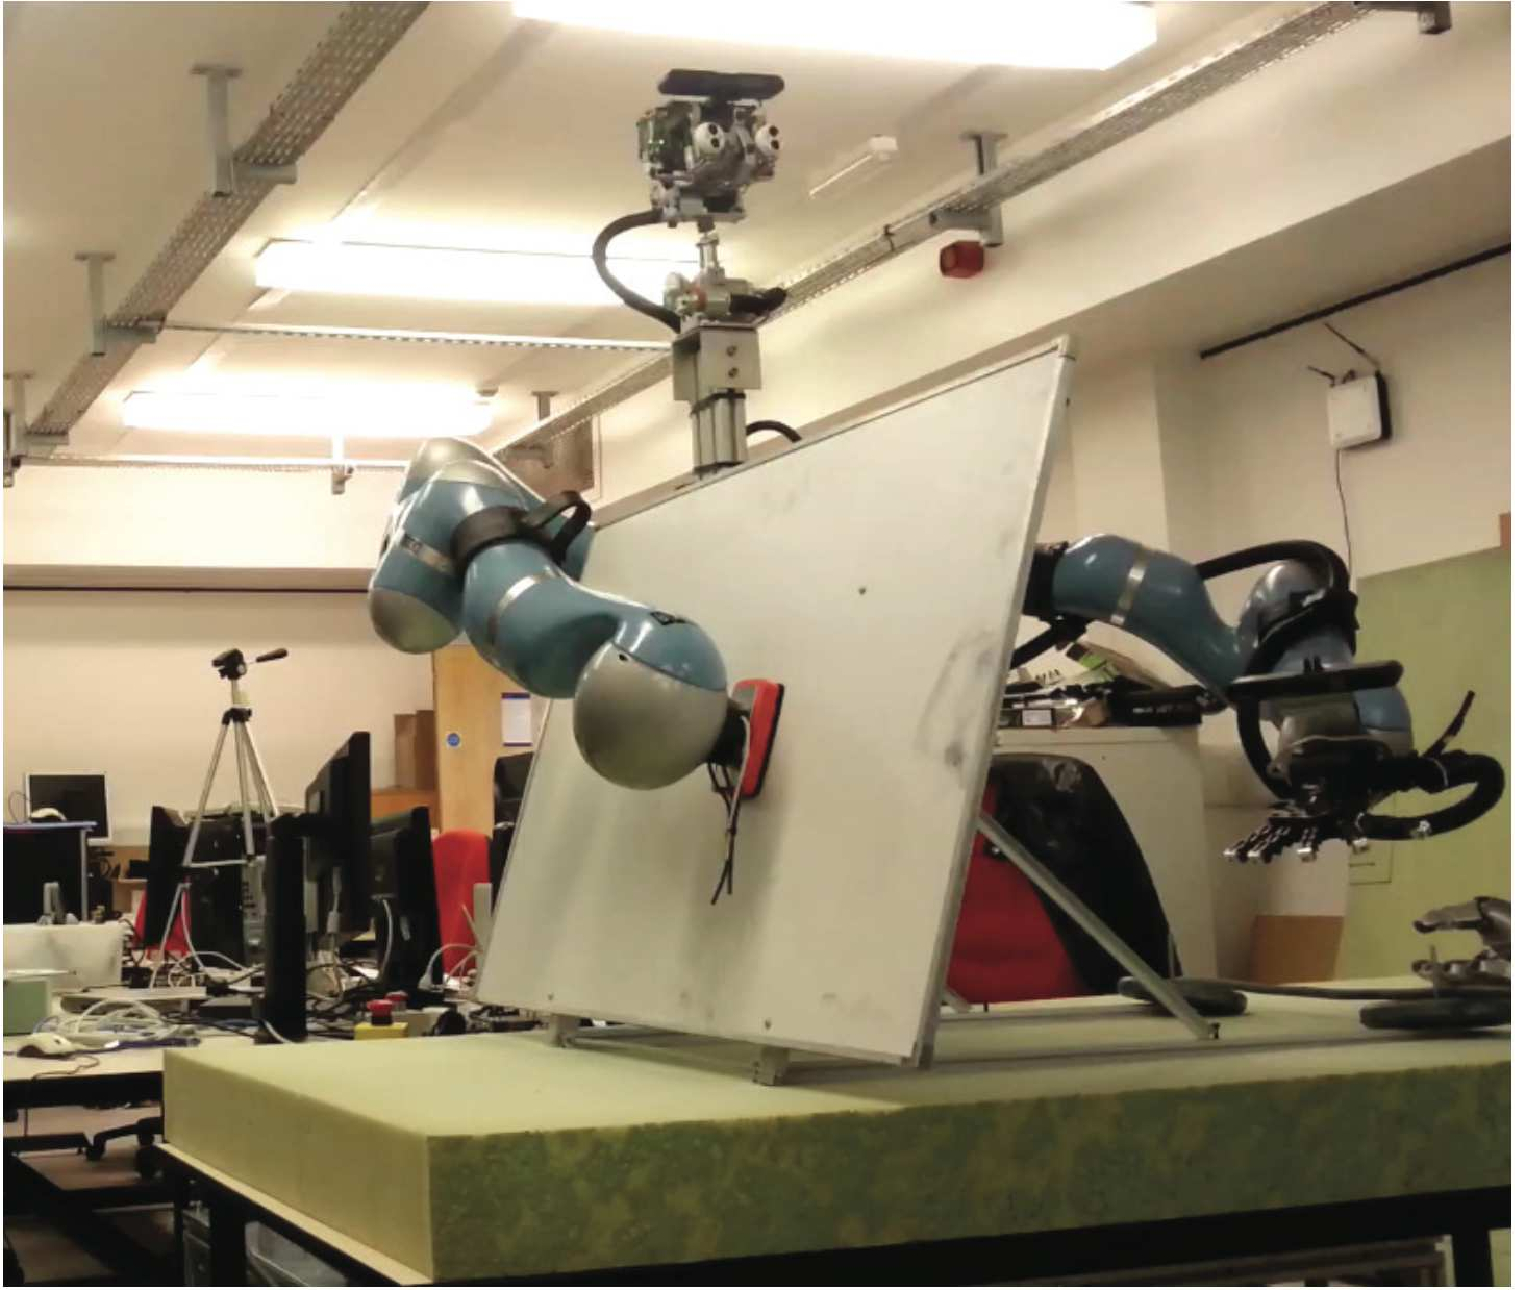
\includegraphics[scale=1]{whiteboard.pdf}
  \caption{Experimental setting. We used the right arm of the humanoid
    platform Boris, and placed the board in between its two arms so that the z
    axis of the robot end effector frame, the z axis of the robot base frame
    and the axis orthogonal to the board are parallel.}
  \label{whiteboard}
\end{figure}
